% outline background

% 1. Video games
% 2. Reinforcement learning
% 3. Deep Reinforcement Learning
% 4. Conclusion

\chapter{Background}

\section{Reinforcement Learning}

Reinforcement Learning is centered around the idea that a good set of problems
in control learning and artificial intelligence can be viewed as sequential
decision making processes. In such formalisation we consider \emph{agent} all
the parts of the problem that contribute to the execution of the decision-making
process, and \emph{environment} everything outside of the agent. given a
discrete-time setting the full system is commonly framed in the following way:
at every episode $t$ the agent receives some observation $s_t \in S$ and from the
environment and executes an action $a_t \in A$ derived from a policy $\pi : S
\rightarrow A$, and receives a reward $r_{t+1} \in \mathbb{R}$. The objective of
reinforcement learning algorithms usually consist in maximising the reward
received in a certain time frame using the experience gained by acting within
the environment. 

\subsection{Markov Decision Processes}

The decision process becomes quickly intractable if you have to process the
entirety of the experience at every step, therefore we need a system that allows
us to approximate history without losing information.

We define \emph{Markov Decision Process} (MDP) a task where the current
observation and reward depend only on the past observation-action pair.

\begin{equation}
Pr(s_{t+1}, r_{t+1} | s_1, a_1, ... , s_t, a_t) = Pr(s_{t+1}, r_{t+1} |
s_t, a_t)
\end{equation}

The observed state $s_t$ is called the \emph{Markov State}, and is defined as
the state that summarises all gained experience up until time $t$. If during a
particular task all the agent observes are Markov states, then the problem is
defined \emph{fully observable}, otherwise it's \emph{partially observable}. Our
work focuses on fully observable problems, but we will take partial
observability into account towards the final chapters to discuss some of the
properties of this particular subset of tasks. Additionally we assume our task
to be \emph{episodic}, which means that the a finite horizon with a number of
reachable terminal states, and that the environment and the agent have finite 
action and state spaces $A$ and $S$.

In general MDPs define a transition probability $P_a(s, s')$ describing the
probability that the process might move into a new state $s'$ from state $s$
taking action $a$, and a reward function $R_a(s, s')$ that provides the expected
reward for such transition.

\begin{equation}
P_a(s, s') = Pr(s' | s, a)
\end{equation}
\begin{equation}
R_a(s, s') = \mathbb{E}[r|s, s', a]
\end{equation}

At every step the action taken by the agent is selected by a policy $\pi(s, a) =
P_r(a | s)$, and we know that any given MDP there exist an optimal policy
$\pi^*(s, a)$ that maximises the expected total reward $R_t = \sum^T{r_t}$:

\begin{equation}
  \pi^*(s, a) = \operatornamewithlimits{argmax}_{\pi} \mathbb{E}_{\pi}[R_t | s_t]
\end{equation}

Reinforcement learning methods can finally also be divided in two groups with
respective to whether or not they model $P_a(s, s')$ and $R_a(s, s')$.
\emph{Model-free} reinforcement learning learn from experience without any
knowledge of environment, \emph{model-based} reinforcement learning either
assume some or full knowledge of the environment or estimate it during the
learning process.

Some of the most successful and popular reinforcement learning algorithms are
based on the idea of choosing actions depending on the \emph{value} of current
and future states. We define $V_{\pi}(s)$ and $Q_{\pi}(s, a)$ to be respectively
the expected return from state $s$ under a policy $\pi$ and the expected return
after choosing an action $a$ in $s$ before following $\pi$.

\begin{equation}
V_{\pi}(s) = \mathbb{E}[R_t | s]
\end{equation}
\begin{equation}
Q_{\pi}(s, a) = \mathbb{E}[R_t | s, a]
\end{equation}

Depending on the algorithm, either or both functions are updated iteratively as
new observations arrive. They can then be taken as factors into the planning
process by simple greedy policies or more complex agent systems.

% insert some examples of model-free and model-based models

All of those models unfortunately do not scale well when tackling large or
growing action spaces, as the framework itself suffers from the so-called
\emph{curse of dimensionality}. 

\subsection{Hierarchical Reinforcement Learning}

It has been shown that planning methods can
strongly benefit from including some form of hierarchical modelling, however
most classical reinforcement learning algorithms do not naturally offer a way to
incorporate hierarchies into their pipelines.

Many researchers have tried to experiment with several methods for hierarchical
reinforcement learning. Contributions have explored with changing different part
of the standard reinforcement learning process, but they have mostly focused on
adding temporal abstractions. These abstractions have for instance been used to
create forms of \emph{temporally-extended actions} such as 
\emph{behaviours},
\emph{skills}, 
\emph{options}, 
or \emph{control modes}.
Those methods involve splitting and clustering states in some way to allow
the creation of partial policies, which can then be combined using Bayesian
reasoning or some other type of control (even RL itself).

% maybe explain SMDP here

Another similar approach to the problem is value decomposition methods such as
MAXQ, a hierarchy of sub-tasks in learnt and concurrently solved by decomposing
the graph until primitives are reached. The higher layers are governed by the
policy, but the available actions reduce as the algorithm walks the graph.

% Put MAXQ graph

\subsection{Deep Reinforcement Learning}

Deep Reinforcement Learning aims to solve the problem of learning policies from
multi-dimensional state representations without having to manually engineer
features and the representation itself. Reinforcement learning has historically
made use of general state approximators like Artificial Neural Networks (ANNs),
but difficulties in training multi-layer architectures and the additional
learning time has stopped researchers from being able to solve the
state-engineering problem and focus purely on tackling the decision-making part.
The recent surge of Deep Learning has managed to shake the reinforcement
learning community and try to use newly developed architectures as powerful
general state approximators.

\subsubsection{Deep Learning}

Deep learning has received an increasing amount of attention in recent years.
Its usage has given rise to several powerful generative and discriminative
models that have resulted in groundbreaking performances in various applied
machine learning tasks such as speech processing, object recognition, machine
translation and more generic data analysis.

The strength of deep learning models - when compared to standard ``shallow''
approaches in machine learning - consists in the ability to concurrently learn
multiple representation of some input space, therefore allowing to effortlessly
construct models that can learn to automatically detect and extract features.
Different architectures and stacks of layers can allow to process visual input,
language sentences, raw motor data and many more dimensionally complex input
spaces.

The main issue with those new models is that they require a lot of data to
converge to a good internal representations even with modern and specialised
optimisation algorithms, however reinforcement learning generally suffers from
the same issue, which makes the two techniques relatively compatible.

We'll see in Chapter 3 that by employing some learning tricks it is in fact possible
to use deep networks to approximate a lot of the classic reinforcement learning
functions (such as for instance the value function $V_{\pi}(s)$).
% DQN goes into methodology

\section{Research using games}

\subsection{ALE}

\subsection{RTS AI Research}

\begin{figure}[h]
    \centering
    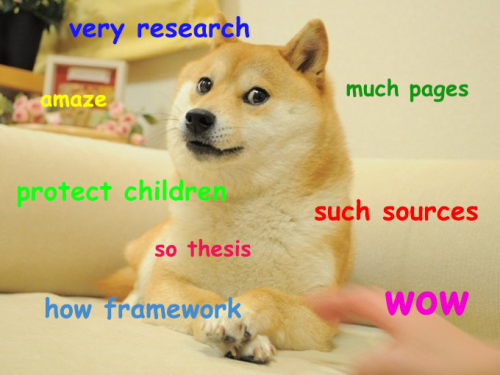
\includegraphics[width=\textwidth]{placeholder}
    \caption{0 A.D., an open source cross-platform Real-Time Strategy game.}
    \label{fig:ALE}
\end{figure}


Real time strategy (RTS) games have historically been a source of complex
problems for AI researchers. The domain they represent is essentially a
simplified military simulation where players fight live and fight in a
fixed-size 2D map for the control of the resources lying all over the map to
build armies and an economy that allows them to win battles and finally the
overall game. The variety of AI and decision problems that this typology of
games involves and requires solving include (but are not limited to):

\begin{itemize}
  \item Decision making under uncertainty
  \item Opponent modelling and Learning
  \item Resource management
  \item Real-time planning
  \item Exploration/exploitation dilemma
\end{itemize}

Those are all terribly challenging problems that have spawned several techniques
and even entire fields of research \citep{buro2003real}. The creation of a machine
learning system that can at least partially solve all those problems and
therefore have the chance to be able to play with a human opponent is far from
being close, even with the relatively game-changing performances of Deep
Reinforcement Learning.

In the past years several RTS research platforms have emerged, the most
prominent ones being Stratagus, OpenRTS and Wargus, however the lack of polish,
missing game mechanics and features that are normally available in commercial
RTS games and lack of community does not make them ideal to do AI research,
especially now that some important parts of it rely also on good amounts of
available data to be fruitful. A more feasible solution was instead to take one
of the popular commercial games and adapt it as to make it an AI testing suite;
in our case, we chose the most popular RTS game every developed: StarCraft.

\subsection{StarCraft Brood War}

Starcraft is a relatively old commercial game developed in 1998 by Blizzard
Entertainment, Inc. that represents the quintessence of Real Time Strategy
games. Since the beginning it has attracted tens of millions of players, selling
as many copies and pioneering the use of videogames as competitive e-sport
platforms. As a consequence StarCraft has been used as a platform for
professional competitions for nearly 20 years, generating annually an industry
of several millions of US dollars. When StarCraft 2 was released in 2009, the
game sold even more copies, generating another wave of popularity for online
gaming that as now has yet to stop growing. With such a background it should be
clear why it's important to provide the artificial intelligence and machine
learning community a way to use the massive amount of collected playing data
available online to start seriously tackling the complexity of Real-Time
Strategy games.

Its code is unfortunately completely closed and Blizzard have never
really opened the game to modifications, but luckily a few users have developed
a system to read and modify the memory of the game, called Brood War Application
Programming Interface (BWAPI)\cite{bwapi2011brood}.

\begin{figure}[h]
    \centering
    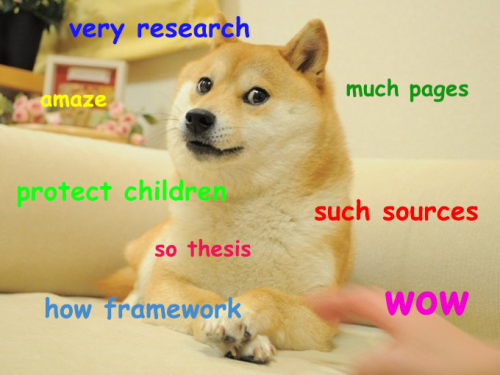
\includegraphics[width=\textwidth]{placeholder}
    \caption{Typical in-game screen of a StarCraft Brood War match.}
    \label{fig:ALE}
\end{figure}

\subsubsection{RTS AI Competitions}

RTS games have recently become popular within the AI research community
due to their challenging properties. With the goal of eventually beating pro-
fessional human players at popular RTS games like starcraft, several RTS
AI competitions have been created to foster competition and help improve the
state-of-the-art. The first such competition took place in 2006 [11] with the de-
velopment of the Open RTS (orts) [12] program at the University of Alberta.
These competitions had several categories focusing on important sub-problems
in RTS games such as resource gathering and small-scale combat.
4With the release of the BroodWar Application Programming Interface
(BWAPI) [39] in 2009, it became possible to control the popular retail game
of starcraft using C++ programs. In 2010 the first starcraft AI Com-
petition was organized by Ben Weber at the University of California, Santa
Cruz as part of the AIIDE conference, and since 2011 it has been organized
and run annually at the University of Alberta. Two other major starcraft
AI Competitions have arisen since then, namely the Computational Intelli-
gence in Games (CIG) Competition, as well as the Student starcraft AI
Competition (SSCAI) [15]. These competitions have focused on playing the
full game of starcraft with no cheats or hacks allowed, bots must face the
same harsh real-time conditions that human players face. These competitions
have motivated many people to join the RTS AI community including both
academics and hobbyists alike.

\section{Summary}

The first part of this chapter has presented the Reinforcement Learning
framework and the Markov Decision Process, a formalisation of decision-making
tasks that allows to study, analyse and compare reinforcement learning
algorithms. In particular we have reviewed work in model-free reinforcement
learning, and we have looked at research focused on adding some form of
hierarchical structure to reinforcement learning as a way to address the problem
of learning growing policy spaces. Additionally we have looked at recent work
that addresses the problem of learning policies from visual information using
deep learning, a powerful set of algorithms for building generative models that
can automatically discover features and that work surprisingly well for domains
when lots of data is available.

The second part of the chapter has focused on reviewing some of the available
video-game platforms that have successfully been used in artificial intelligence
research, looking in particular at Real-Time Strategy games. Finally we have
provided a description of StarCraft, its properties and the rationale behind the
idea of transforming it into a fully-fledged agent learning platform.
